\let\negmedspace\undefined
\let\negthickspace\undefined
\documentclass[a5paper,10pt]{article}
\usepackage[margin=10mm]{geometry}
%\usepackage{lmodern} % Ensure lmodern is loaded for pdflatex
\usepackage{tfrupee} % Include tfrupee package

\setlength{\headheight}{1cm} % Set the height of the header box
\setlength{\headsep}{0mm}     % Set the distance between the header box and the top of the text

\usepackage{gvv-book}
\usepackage{gvv}
\usepackage{cite}
\usepackage{amsmath,amssymb,amsfonts,amsthm}
\usepackage{algorithmic}
\usepackage{graphicx}
\usepackage{textcomp}
\usepackage{xcolor}
\usepackage{txfonts}
\usepackage{listings}
\usepackage{enumitem}
\usepackage{mathtools}
\usepackage{gensymb}
\usepackage{comment}
\usepackage[breaklinks=true]{hyperref}
\usepackage{tkz-euclide} 
\usepackage{listings}
% \usepackage{gvv}                                        
\def\inputGnumericTable{}                                 
\usepackage[latin1]{inputenc}                                
\usepackage{color}                                            
\usepackage{array}                                            
\usepackage{longtable}                                       
\usepackage{calc}                                             
\usepackage{multirow}                                         
\usepackage{hhline}                                           
\usepackage{ifthen}                                           
\usepackage{lscape}
\usepackage{circuitikz}



\author{EE25BTECH11041-Naman Kumar }
\graphicspath{./figs/}

\begin{document}
\begin{center}
    \huge{12.54}\\
    \large{EE25BTECH11041 - Naman Kumar}
\end{center}
Question:\\
For a matrix
\begin{align}
    \vec{M}=\begin{pmatrix}
        \frac{4}{5} & -\frac{3}{5} \\\frac{3}{5} & x
    \end{pmatrix}
\end{align}
the transpose of the matrix is equal to the inverse of the matrix, i.e., $\vec{M}^T=\vec{M}^{-1}$.The value of x is given by\\
\solution \\
\begin{align}
    \vec{M}^T=\vec{M}^{-1} \label{1}
\end{align}
Multiple $\eqref{1}$ with $\vec{M}$
\begin{align}
    \vec{M}\vec{M}^T=\vec{I}
\end{align}
$\vec{M}$  is orthogonal matrix
\begin{align}
\begin{pmatrix}\frac{4}{5} & \frac{-3}{5} \\ \frac{3}{5} & x\end{pmatrix}\begin{pmatrix}\frac{4}{5} & \frac{-3}{5} \\ \frac{3}{5} & x\end{pmatrix}^T=\begin{pmatrix}1&0\\0&1\end{pmatrix}\\
\begin{pmatrix}\frac{16}{25}+ \frac{9}{25} & \frac{-12}{25}+\frac{3x}{25} \\ \frac{-12}{25} +\frac{3x}{25} & \frac{9}{25}+x^2\end{pmatrix}=\begin{pmatrix}1&0\\0&1\end{pmatrix}\\
\frac{-12}{25}+\frac{3x}{25}=0\\
x=\frac{4}{5} \label{2} \\ 
\frac{9}{25}+x^2=1\\
x^2=\frac{16}{25}\\
x=\pm \frac{4}{5} \label{3}
\end{align}
from $\eqref{2}$ and $\eqref{3}$
\begin{align}
    x=\frac{4}{5}
\end{align}
\begin{figure}[H]
    \centering
    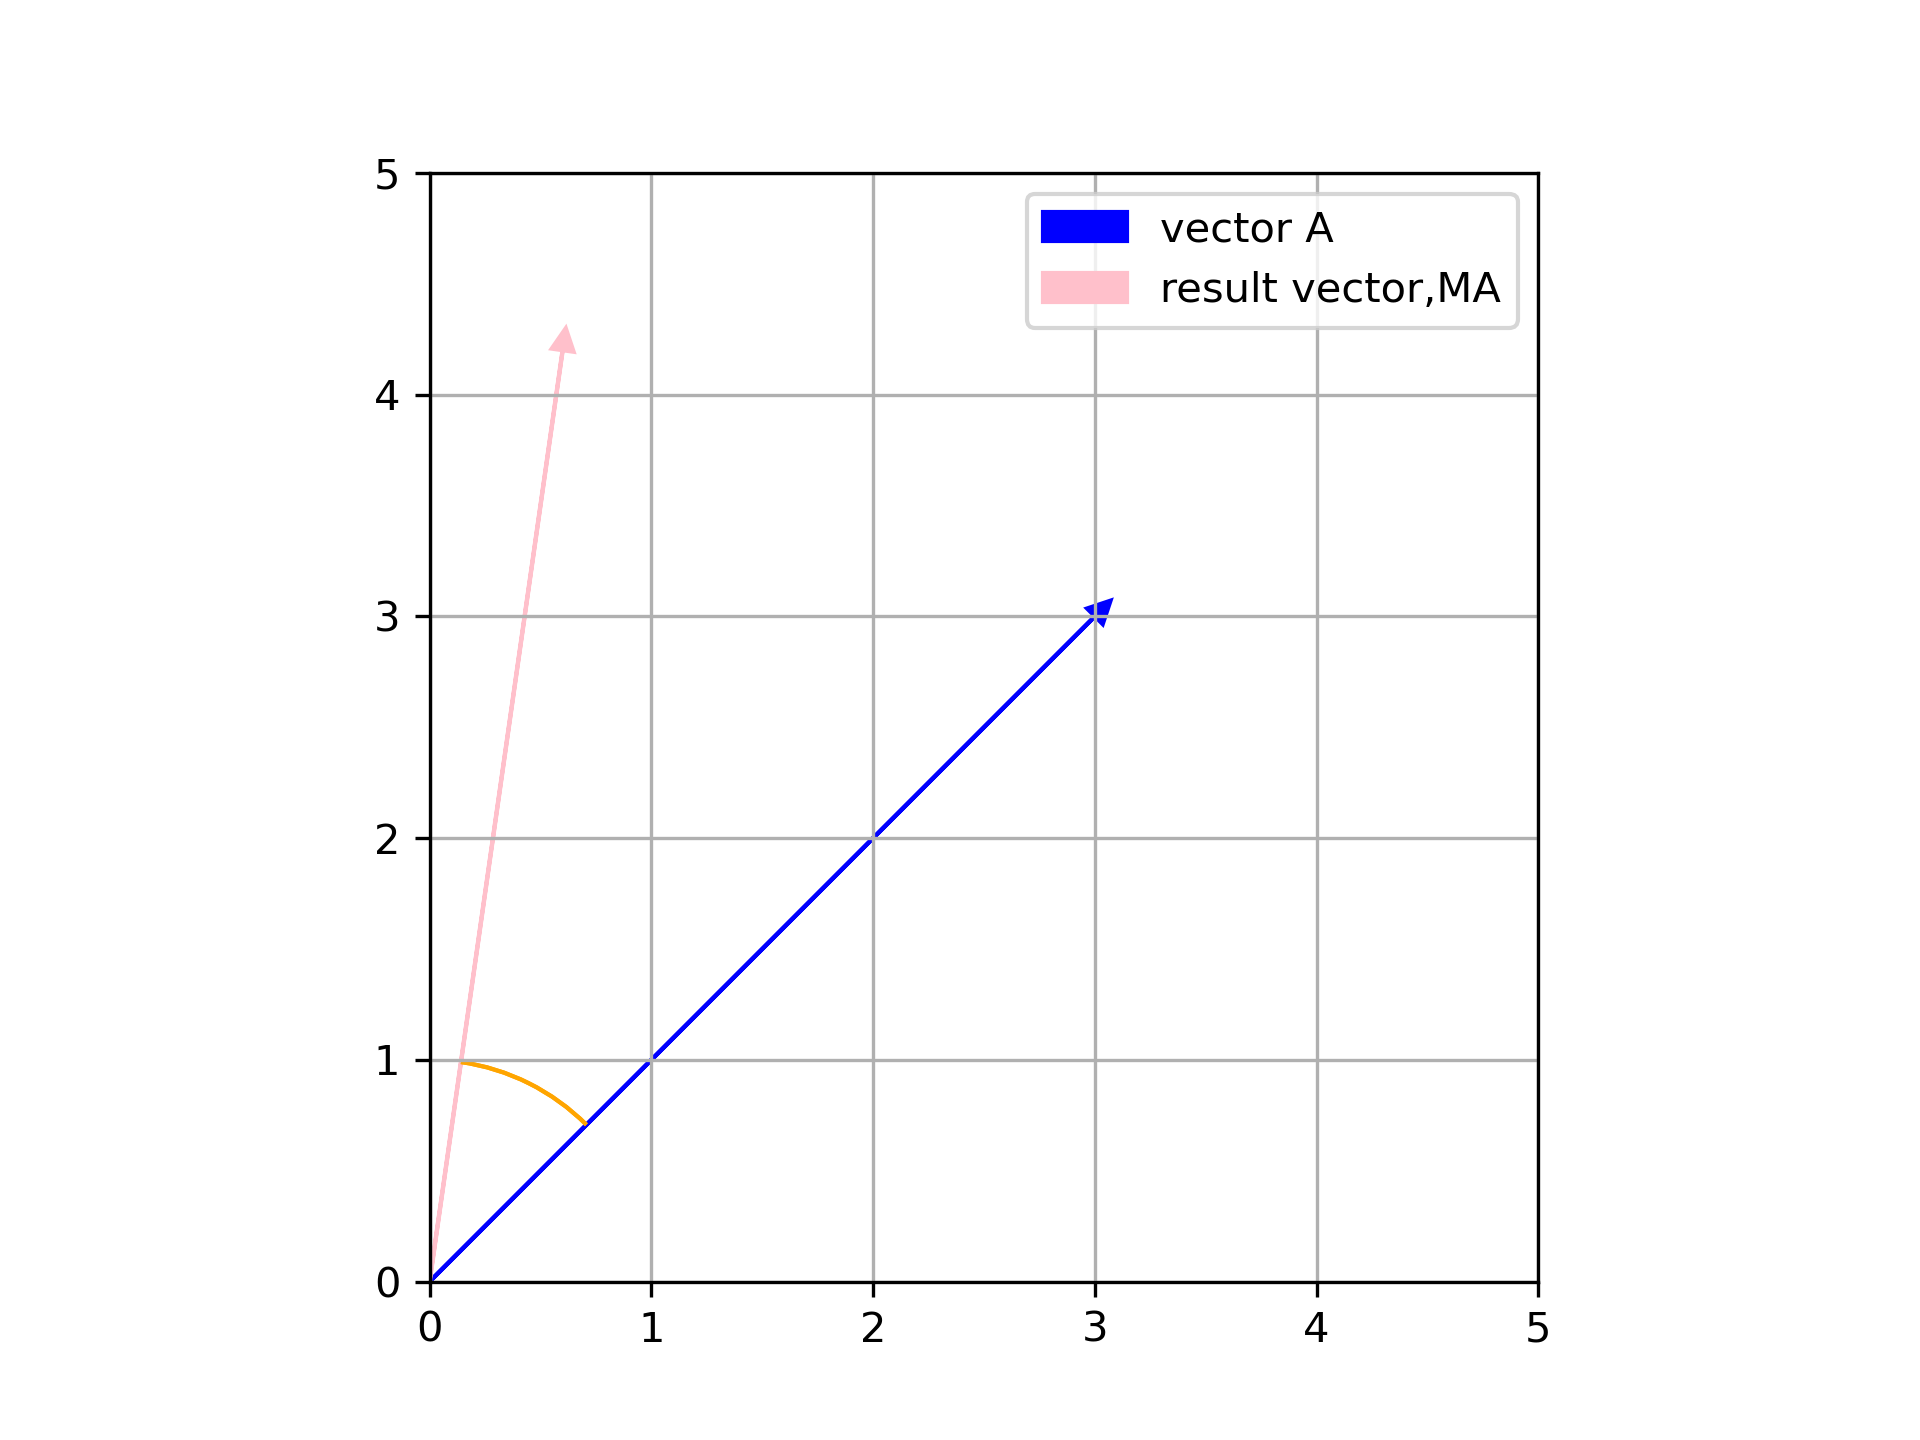
\includegraphics[width=0.7\columnwidth]{figs/fig1.png}
    \caption{}
    \label{fig:placeholder}
\end{figure}
\begin{figure}[H]
    \centering
    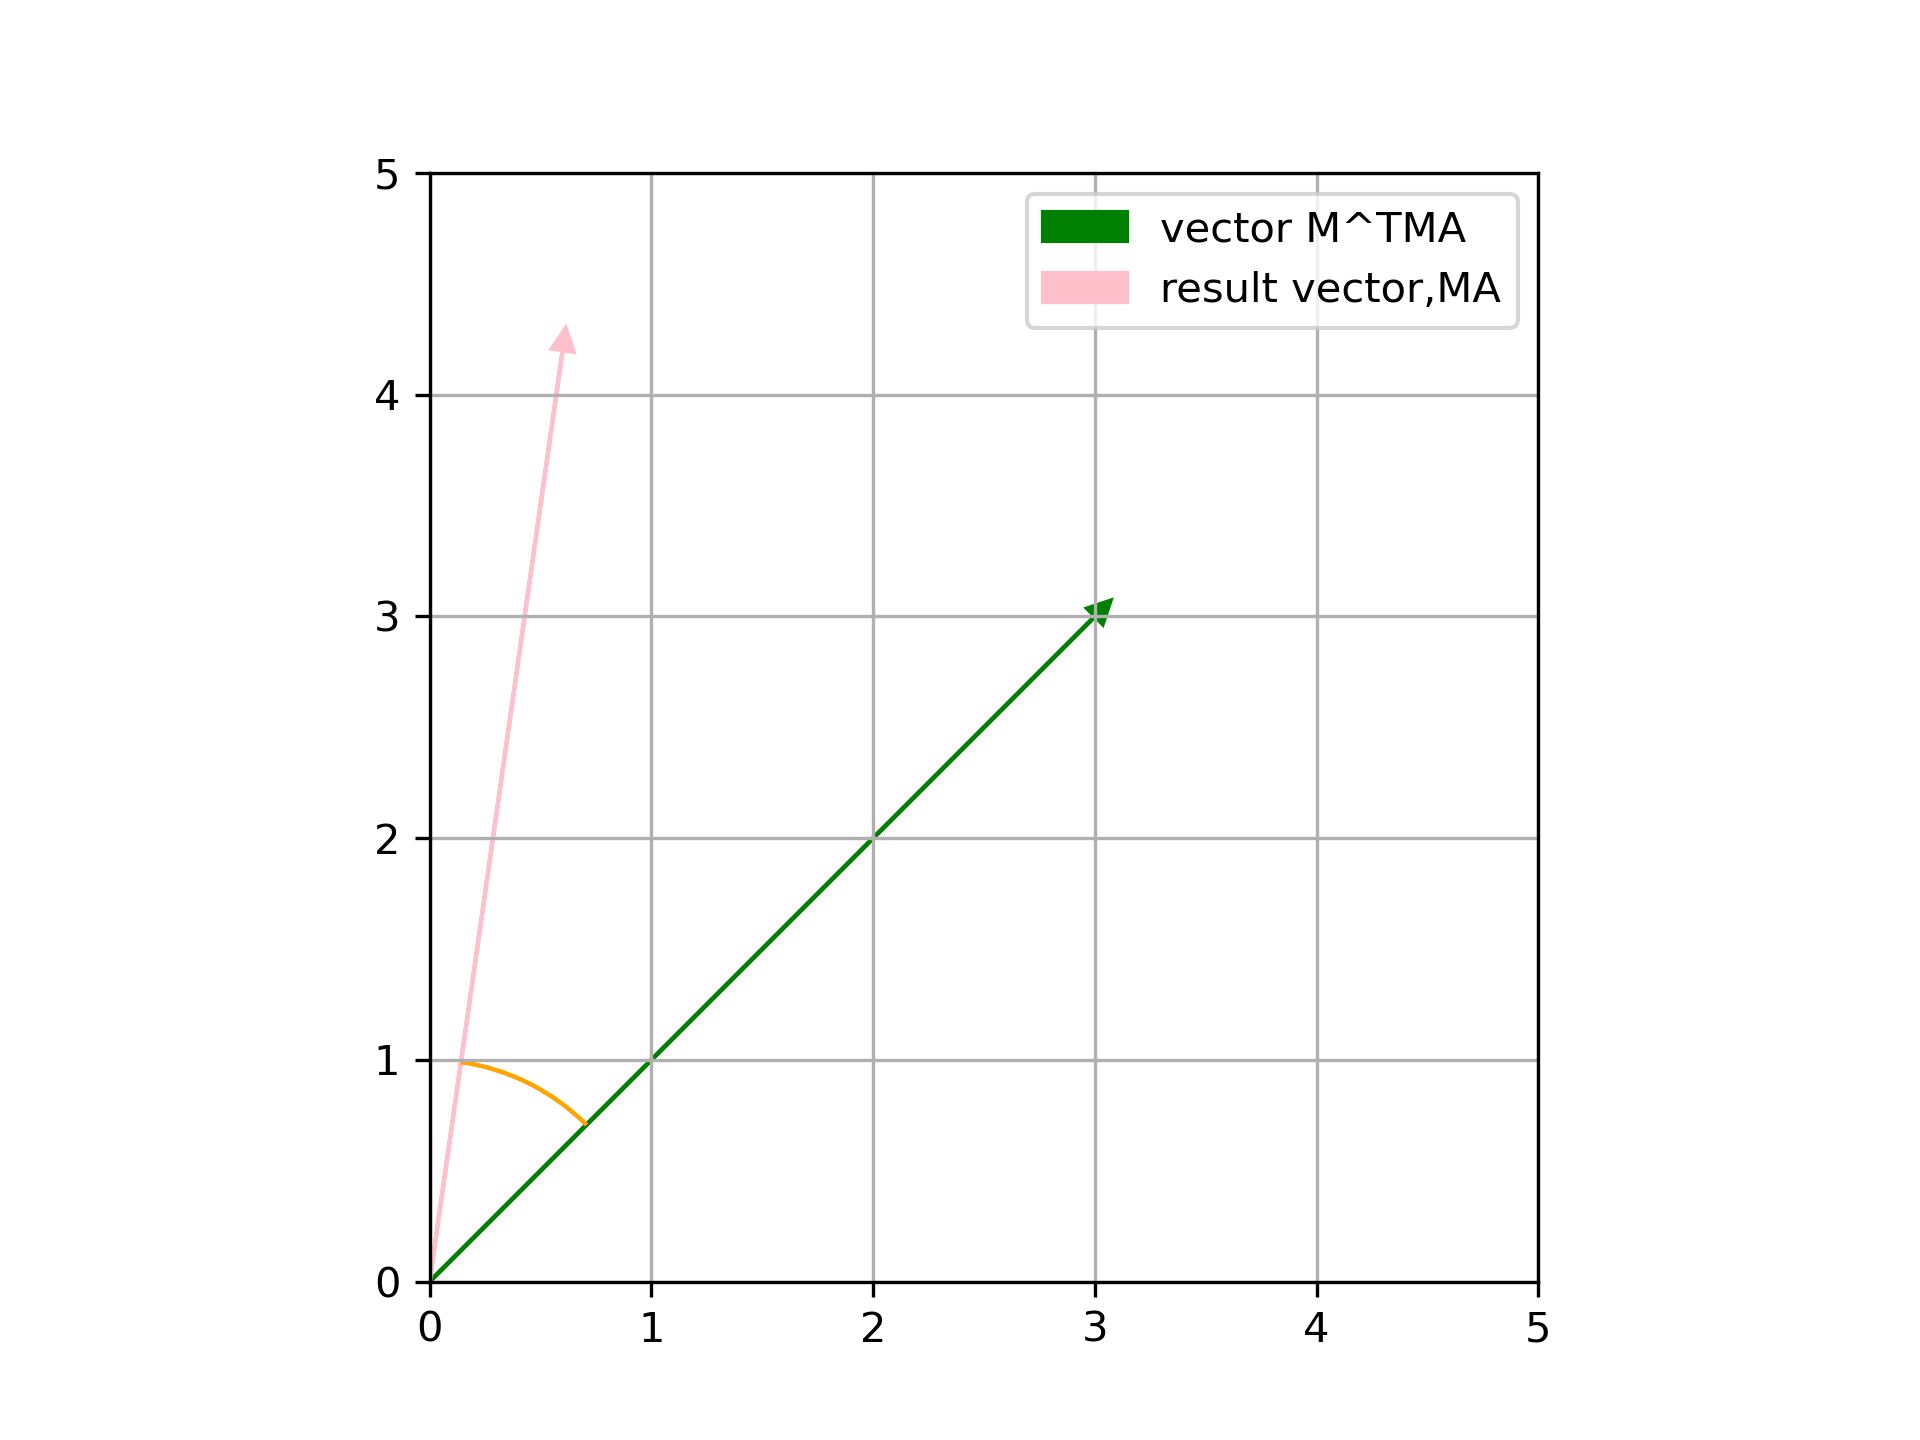
\includegraphics[width=0.7\columnwidth]{figs/fig2.png}
    \caption{}
    \label{fig:placeholder}
\end{figure}
\end{document}
